\section{Durchführung}
\label{sec:Durchführung}
\begin{figure}
  \centering
  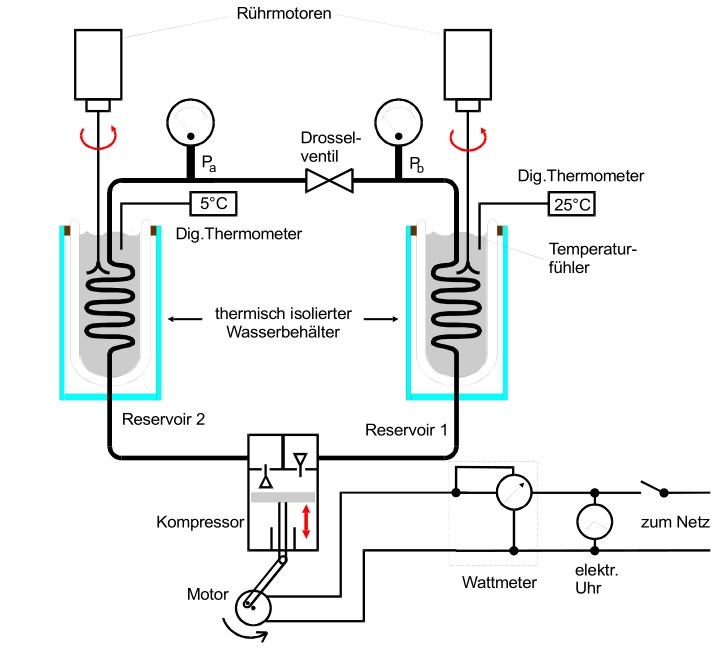
\includegraphics{data/Abb2.jpg}
  \caption{Apparatur zur Messreihe. \cite{AnleitungV206}}
  \label{fig:Abb2}
\end{figure}
Zuerst sind Anfangsdrücke, Temperaturen, sowie die spezifische Wärmekapazität des Kupfers aufzunehmen.
Danach werden die Behälter mit 4 Liter Wasser gefüllt und die Rührmotoren eingeschaltet.
Dann wird der Kompressor angeschaltet und es werden fortan im Minutentakt die Messdaten der Mano- und Thermometer, sowie die Zeit und Leistungsaufnahme des Kompressors notiert.
Diese Messreihe wurde fortgeführt bis beim zu eritzenden Reservoir eine Temperatur von $50^\circ\text{C}$ erreicht wurde.
Für die Auswertung sind nun die Güteziffer, der Massendurchsatz $\frac{dm}{dt}$ und der Wirkungsgrad zu bestimmen.